\chapter{\label{ranking-algorithms}Ranking algorithms}

\section{What problem do a ranking algorithm solve?}


The main purpose of the algorithms discussed below in this section is to answer the question \emph{Given a score, what is the rank of a user or item with this score?}. The opposite question -- \emph{Given a rank, what is the score for this rank?} is very similar but not adressed here directly even though most approaches to the ranking problem indirectly answers that question too.

\todo{How to be more formal about this?}
\todo{
  Make reference to \href{http://googleappengine.blogspot.se/2009/01/google-code-jams-ranking-library.html}{Google Code Jam's Ranking Library Released}}

\section{What is ranking?}

\begin{shaded}
  
  What is ranking, formal definition
 
The rank of a well-founded set is defined inductively as the smallest ordinal number greater than the ranks of all members of the set.[1] In particular, the rank of the empty set is zero, and every ordinal has a rank equal to itself.
\href{https://en.wikipedia.org/wiki/Von\_Neumann\_universe}{Wikipedia - Von Neumann universe}

Well founded relation:

$\forall S \subseteq X ( S \neq \varnothing \rightarrow \exists m \in S \forall s \in S (s, m) \notin R)$ \href{https://en.wikipedia.org/wiki/Well-founded\_relation}{Wikipedia - Well-founded relation}

Define ordinal (each ordinal is the well-ordered set of all smaller ordinals?)

\end{shaded}

\subsection{Types of ranking algorithms}

Ranking algorithms can coarsely be divided in two categories: \emph{exact} and \emph{approximating} algorithms. The exact algorithms deal with the ranking problem by sorting and counting. The sorting part is commonly accomplished by indexing the score-property of the entity or the corresponding column in a table in case a relational database is used.  

As mentioned in the introduction, obtaining an exact rank may not be necessary. Other considerations such as speed and cost may be more important. Approximating algorithms estimate the rank by linear interpolation within a segement of ranks. Suitable segments may be found with an \emph{offline-method} such as scanning all scores periodically keeping track of scores at the segments boundaries or with an \emph{online-method} with a \emph{streaming algorithm} that maintains a model for estimating ranks by continuosly updating a number of statistical measures.

\todo{Fix last sentence}

\subsubsection{Stability}

In both cases a sorted list needs to be created. If the chosen sorting algorithm is not stable the ranking will be non-deterministic. This may or may not be a problem depending on the application. 

\section{Exact algorithms}

\subsection{Rank by counting}

The naive approach to getting the rank for a score is to obtain a sorted list from the set of scores. Then start counting elements in that list that scores higher than the score in question.

\begin{shaded}

 \emph{I want to define ranking by counting like this:}

  1. define a set of items, and an item i with score s.

  2. define a sorted list of those items or someway indicate that the set is sorted by some relation

\textbf{either}
  
  3a. assign ordinal numbers to the items \\
  4a. get the ordinal number for the i.

 \textbf{or}

  3b. count items before i

\textbf{or}

  3c. Better way of counting items ``before'' the new item?
  
\end{shaded}

This way of getting the rank can be done with a simple query in SQL
\texttt{SELECT count(id) FROM Highscores WHERE Score > TheScore} or by increasing a counter while iterating through the set of highscores in case a non-relational database is used. In any case the items should be indexed on the highscore-field.

Obtaining rank for a score by this method implies scanning through all items having a score higher than the one you want to obtain the rank for. The time complexity of this approach is obviously $\mathcal{O}(n)$ making it unusable for online applications in terms of cost and response time\footnote{If the ranking function is not required to return a new rank, the actual rank could be assigned periodically by a background job to all the highscores. In this case the $\mathcal{O}(n)$ time complexity would be more tolerable.}.

\subsection{Tree based approach}

As described above, ranking is fundamentally a counting problem. One way to accomplish counting more efficiently is by storing the count of each score in an N-ary tree. Each non-leaf node defines a score range and its associated count and the leaves represents individual items from the value domain, ie discreete scores.

Score updates and getting the rank for a score with this algorithm has a time complexity of $\mathcal{O}(\log{} n)$. However, since fetching or updating a node may be relatively expensive in case it has to be fetched from a database system the number of ranges per node needs to be chosen so that the height of the tree remains reasonable low\footnote{The Google Code Jam Ranking Library uses 100 buckets per node}. The height of the tree is $ceil(log_{rangesize}numscores)$.

A naive solution would result in a space complexity is $\mathcal{O}(m)$ where $m$ is the size of the value domain. 

\todo{If space complexity is a problem, having \emph{buckets} at the leaf-level and do interpolation would help the situation.}

\todo{The Quantile Digest solution essentially solves this problem.}

\begin{figure}[h!]
  \centering
  \caption{Figure \ref{fig:tree} shows an example of how ranking is done by using a tree based approach. To get the rank for score 30, start by adding the counts for scores greater than 30. There is 22 higher scores and rank for score 30 is thus 23.}
  \label{fig:tree}
  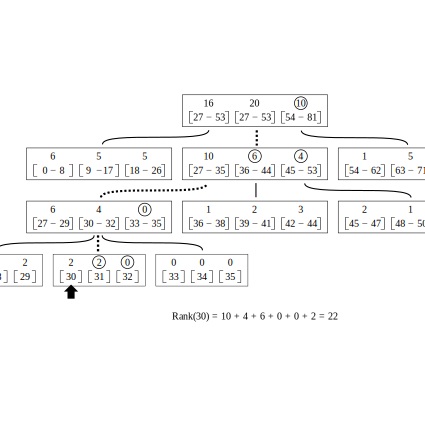
\includegraphics[width=10cm]{img/tree}
\end{figure}

\begin{shaded} There is a lot of practical aspects that needs to be considered when implementing this ranking-algorithm on Google App Engine that are described in detail here
\href{https://cloud.google.com/datastore/docs/articles/fast-and-reliable-ranking-in-datastore/}{Fast and Reliable Ranking in Datastore}. However I don't know if they are especially relevant in this thesis.
\end{shaded}

\section{Approximating algorithms}

Getting an exakt rank for a score may not be crucial. One fairly obvious class of solutions is the ones using linear interpolation of rank within a score range with known ranks at the boundaries.

\todo{IMAGE: Linear interpolation}

\todo{
  Let the true value of a quantity be $x$ and the measured or inferred value $x_0$.
  The relativer error is defined by $\delta x = \frac{\Delta x}{x} = \frac{x_0 - x}{x} = frac{x_0}{x} - 1$, where $\Delta x$ is the absolute error.
  \href{http://mathworld.wolfram.com/RelativeError.html}{mathworld.wolfram.com}
} 



\subsection{\label{bucket}Buckets with Global Query}

The most basic variant of this approach is called \emph{Bucket with Global Query} in the article \href{https://cloud.google.com/datastore/docs/articles/fast-and-reliable-ranking-in-datastore/}{Fast and Reliable Ranking in Datastore}. The same type of algorithm is also in use by the company mentioned in the introduction.

\todo{ ... so I need to mention the company in the introduction.}

A background job periodically scans all highscores, creating a table with entries for scores and corresponding ranks.

The quality of the estimates made by this method depends on several factors.
\textbf{The frequency of the periodic scans} needs to be high enough to keep the error of the estimate at an acceptable level. Also, \textbf{the size of the buckets} have an impact on the result. Yet another factor that are more difficult to deal with is the distribution of the scores within the bucket which can be skewed or simply not very linear within the score range.

\todo{IMAGE: Uneven distribution}

\subsubsection*{Handling error}

A common requirement is that ranking have to be more precise for higher ranks than for lower ranks. This may be accomplished by having small buckets for higher ranks while increasing the bucket size by some formula for the lower ranks. In some cases even an exponential bucket-growth will produce good
enough result. By using this method higher ranks will be predicted with better precision and the bucket-table will stay reasonably small.

However, the method described above may not be enough to handle the highest ranks. One reason for that may simply be that the requirement on the algorithm and ultimately the final solution does not accept approximations \emph{at all} for the top ranks. Also, a wrongly predicted rank will result in a high relative error when dealing with the highest ranks.

\todo{Provide example}

To solve that problem this algorithm can be paired with the \emph{Rank by counting}-algorithm for the highest ranks. This should not be a problem since the underlying highscore data most probably is indexed already. 

\begin{mdframed}[backgroundcolor=red,innerleftmargin=15pt,leftmargin=-10pt,rightmargin=-10pt, innerrightmargin=15pt,innertopmargin=10pt,innerbottommargin=10pt, fontcolor=white, skipabove=20pt, linewidth=0]
  \textbf{Warning! Bumpy road ahead!}
  
  I wish to complete the rest of this chapter for this thesis. It is not essential to my experiments and conclusions later but it provides a completeness to the subject I think would be good.
\end{mdframed}

\subsection{Online approaches, streaming algorithms}

The drawback with the method described above is that the bucket-table after some time will no longer represent the actual distribution of scores and consequently less and less accurate rankings.

An alternative but still similar way of solving the problem could be by estimating a number of quantiles of the distribution of highscores by using a streaming algorithm. 

\emph{Frugal streaming} is a streaming streaming algorithm for estimating a quantile of a stream devised by Ma, Muthukrishnan and Sandler. \cite{frugal_streaming} The algorithm itself is fairly self explanatory (see appendix \ref{frugal}) and have a small memory footprint.

The idea is that by calculating a number of quantiles for every new highscore while keeping track of the total number of highscores you could create a bucket-table as in the algorithm described in section \ref{bucket}.

Calculating exact quantiles of a large dataset is quite expensive.

\subsection{Quantile Digest}

\emph{Quantile Digest} is a tree based stream summary algorithm. The paper that describes the algorithm does it from a sensor network perspective \cite{quantile_digest}.

The algorithm builds a binary tree of the value domain. The tree is then compressed and can be sent to the parent of the sensor. The compression is lossy such that less frequent values are represented as a bucket. The result of the compression is called Quantile Digest.

Quantile query - inverse quantile

\blockquote{

Inverse Quantile: Given a value x, determine its
rank in the sorted sequence of the input values.
175
In this case, we again make the same sorted list (L),
and traverse it from beginning to end. We report the
sum of counts of buckets $v$ for which $x > v.max$ as
the rank of x. The reported rank is between rank(x)
and rank(x) + $\varepsilon$, $rank(x)$ being the actual rank of
$x$.}
